\section{Conclusions}
In this work, we demonstrate and quantitatively analyse one type of spurious responses existing in both linear and non-linear dynamic analysis of vibrating systems that stems from linear interpolation of input load. Within the scope of seismic engineering, typical values are chosen to illustrate the issue. It is worth emphasising that the identified issue exists in all systems as long as linear interpolation is used, regardless of parameters (sampling frequency of input, material properties of system, natural frequency distribution, etc.).

\begin{figure}[htb!]
\centering\footnotesize
\tikzstyle{label}=[rectangle,rounded corners,minimum width=3cm,minimum height=1cm,text centered,draw=black,fill=gray!20]
\tikzstyle{exp}=[rectangle,rounded corners,minimum width=2cm,minimum height=1cm,text centered,draw=black,fill=gray!10]
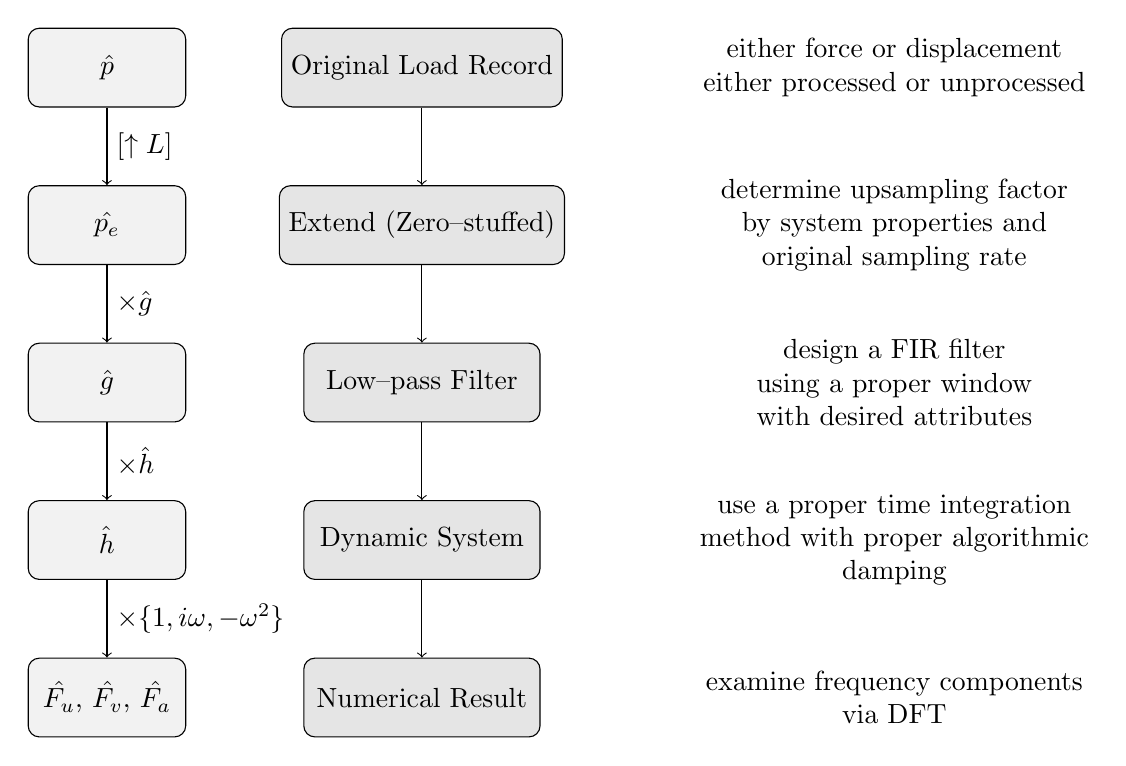
\begin{tikzpicture}
\node(original)[label]{Original Load Record};
\node(extended)[label,below of=original,yshift=-1cm]{Extend (Zero--stuffed)};
\node(filter)[label,below of=extended,yshift=-1cm]{Low--pass Filter};
\node(oscillator)[label,below of=filter,yshift=-1cm]{Dynamic System};
\node(system)[label,below of=oscillator,yshift=-1cm]{Numerical Result};
\draw[->](original)--(extended);
\draw[->](extended)--(filter);
\draw[->](filter)--(oscillator);
\draw[->](oscillator)--(system);
\node[xshift=5cm,right of=original,align=center]{either force or displacement\\either processed or unprocessed};
\node[xshift=5cm,right of=extended,align=center]{determine upsampling factor\\by system properties and\\original sampling rate};
\node[xshift=5cm,right of=filter,align=center]{design a FIR filter\\using a proper window\\with desired attributes};
\node[xshift=5cm,right of=oscillator,align=center]{use a proper time integration\\method with proper algorithmic\\damping};
\node[xshift=5cm,right of=system,align=center]{examine frequency components\\via DFT};
\node(p)[exp,xshift=-5cm,right of=original,align=center]{$\hat{p}$};
\node(pe)[exp,xshift=-5cm,right of=extended,align=center]{$\hat{p_e}$};
\node(g)[exp,xshift=-5cm,right of=filter,align=center]{$\hat{g}$};
\node(h)[exp,xshift=-5cm,right of=oscillator,align=center]{$\hat{h}$};
\node(f)[exp,xshift=-5cm,right of=system,align=center]{$\hat{F_u}$, $\hat{F_v}$, $\hat{F_a}$};
\draw[->](p)--(pe)node[midway,right]{$[\uparrow{}L]$};
\draw[->](pe)--(g)node[midway,right]{$\times\hat{g}$};
\draw[->](g)--(h)node[midway,right]{$\times\hat{h}$};
\draw[->](h)--(f)node[midway,right]{$\times\{1,i\omega,-\omega^2\}$};
\end{tikzpicture}
\caption{typical analysis flow with recommendations}\label{fig:workflow}
\end{figure}

It is evident that the linear interpolation is neither ideal or reliable. The following recommendations are made.
\begin{enumerate}
\item In order to avoid linear interpolation, it is better to have the identical time step size and sampling interval. To this end, analysts shall first choose a proper time step size that would be used in numerical analysis, typically it is smaller than sampling interval and is determined by the property of the dynamic system of interest. Then, the seismogram shall be processed by upsampling. A low--pass filter with sufficiently small side lobe level shall be applied to suppress any components above the Nyquist frequency.
\item The high frequency noise exists intrinsically and can be spotted analytically. Algorithmic damping can alleviate the issue but only to a limited degree, nevertheless, it is still beneficial to adopt a time integration method with adjustable algorithmic damping. In this regard, the de facto Newmark method with average constant acceleration ($\gamma=0.5$ and $\beta=0.25$), which is widely used in seismic engineering, is not recommended.
\end{enumerate}

Based on the above recommendations, the following workflow is proposed, which is also summaries in \figref{fig:workflow}.
\begin{enumerate}
\item Determine whether the seismograph, in the form of either displacement or acceleration, is properly processed. Typical seismographs are preprocessed by applying a band--pass filter with bounds at around \SI{0.05}{\hertz} and \SIrange{25}{50}{\hertz} for structural analysis \citep[see, e.g.,][]{Houtte2017}.
\item Determine a proper time step size and thus the corresponding upsampling ratio.
\item Design a proper upsampling filter so that time step size matches upsampling interval.
\item Avoid high frequency modes in the target structure. Constraints are better implemented via the Lagrange multiplier method.
\item Perform analysis using a time integration method with adjustable algorithmic damping.
\item Examine final results to ensure there is no significant high frequency components.
\end{enumerate}

The numerical examples are carried out using \texttt{suanPan} \citep{Chang2022}. Scripts to generate figures and models can be found online.\footnote{\url{https://github.com/TLCFEM/dsp-dynamics}}